\chapter{Аналитический раздел}

\section{Анализ существующих решений}

Среди уже существующих проектов, решающих поставленную задачу, были выделены 3 аналога (таблица \ref{decisions}) -- сервисы <<HYPE Hackathon Solution>>~\cite{hype}, <<EventTornado>> \cite{eventornado} и <<Hackathon Manager>> \cite{hack_manager}. Данные приложения, позволяют создавать хакатоны, добавлять в них участников, а также получать подробную инфографику по их результатам. Сравнение (приведено в таблице \ref{decisions}) проводилось по ряду критериев: типу приложения, доступности в РФ, стоимости и наличию API.

\begin{table}[H]
	\centering
	\caption{-- Существующие решения поставленной задачи}
	\label{decisions}
	\begin{tabular}{|p{2.3cm}|p{3.3cm}|p{3cm}|p{3cm}|p{3.1cm}|}
		\hline
		\textbf{Название проекта} & \textbf{Тип приложения} & \textbf{Доступ- ность в РФ} & \textbf{Стоимость} & \textbf{Наличие API}\\
		\hline 
		\textbf{HYPE Hacka- thon Solution} & Desktop/Web & Нет & До 50 000\$ в год в зависимости от конфигурации и числа пользователей & Да\\
		\hline
		\textbf{Evento- rnado} & Web & Нет & от 8\$ за пользователя & Нет\\
		\hline
		\textbf{Hacka- thon Manager} & Web & Да & Бесплатно & Нет  \\
		\hline
	\end{tabular}
\end{table}

Из сравнения видно, что <<Eventornado>> и <<Hackathon Manager>> не имеют API и не могут взаимодействовать с другими приложениями. <<HYPE Hackathon Solution>> же обладает относительно высокой стоимостью и недоступна на территории РФ. В данной работе была произведена попытка нивелировать недостатки конкурентов и в то же время совместить их преимущества.

\section{Анализ предметной области}

Как уже было сказано, хакатоны - это мероприятия, в которых программисты соревнуются в решении задач за ограниченное время. Каждое событие сфокусировано на конкретной области, такой как разработка приложения, API либо анализ данных. Основная часть хакатона - это время, которое участники проводят над своими проектами. Обычно это от 24 до 72 часов, в зависимости от конкретного хакатона. В это время участники работают в командах, создавая и развивая свои проекты в соответствии с заданием хакатона или своими собственными идеями \cite{skillfactory}.

Главной особенностью данного типа мероприятий является то, что по окончании соревнования, команды должны представить законченный программный продукт. Жюри, как правило, состоит из экспертов в области разработки, бизнеса или другой отрасли, связанной с тематикой хакатона. Жюри оценивает проекты, созданные участниками, и выбирает лучшие из них на основе определенных критериев, таких как инновационность, полезность, применимость, дизайн и технические навыки. Часто жюри также задает вопросы участникам, чтобы лучше понять их проекты и принять более обоснованные решения. Кроме того, в ходе хакатона участники могут получать обратную связь от жюри и других участников, что помогает им улучшить свои навыки и подготовиться к будущим мероприятиям \cite{hackai}. 

\section{Формализация задачи}

В ходе выполнения курсовой работы необходимо разработать базу данных для хранения и обработки данных о проводимых хакатонах, командах, принимающих в них участие, а также непосредственно участниках. Кроме того, необходимо реализовать возможность участникам присоединяться к командам, организаторам хакатонов - создавать мероприятия. Также нужно добавить возможность отслеживать рейтинг команд и отдельных участников. Для каждой категории пользователей необходимо реализовать различный функционал и предоставить им определённый набор прав.

\section{Формализация данных}

В ходе анализа предметной области были выделены следующие сущности:
\begin{itemize}
    \item хакатон, обладает следующими полями: id, название, дата проведения, тематика, id организатора,  длительность и id команд, занявших 1-е, 2-е и 3-е место;
    \item команда, имеет поля: id, id капитана, число участников, название, рейтинг; 
    \item участник, обладает полями: id, логин, пароль, имя и рейтинг;
    \item организатор, обладает полями id, имя, логин, пароль;
    \item администратор, имеет поля id, имя, логин, пароль;
    \item заявка, имеет поля: id, тип, статус, id подавшего, тип учетной записи подавшего, название хакатона/команды (в зависимости от типа заявки), поле для комментария.
\end{itemize}

Кроме того, были выделены следующие вспомогательные таблицы, содержащие лишь одно поле id:
\begin{itemize}
    \item тип заявки, может принимать следующие значения: 
    \begin{itemize}
        \item 1 -- создание команды;
        \item 2 -- создание хакатона;
        \item 3 -- вступление в команду;
        \item 4 -- участие в событии.
    \end{itemize}
    \item тип учетной записи подавшего: 1 - участник, 2 - организатор;
    \item статус заявки:
    \begin{itemize}
        \item 1 -- открыта;
        \item 2 -- в работе;
        \item 3 -- принята;
        \item 4 -- отклонена.
    \end{itemize}
    \item тип учетной записи пользователя.
    
\end{itemize}

ER-диаграмма сущностей предметной области представлена на рисунке \ref{er-diagram}.

\begin{figure}[H]
	\begin{center}
		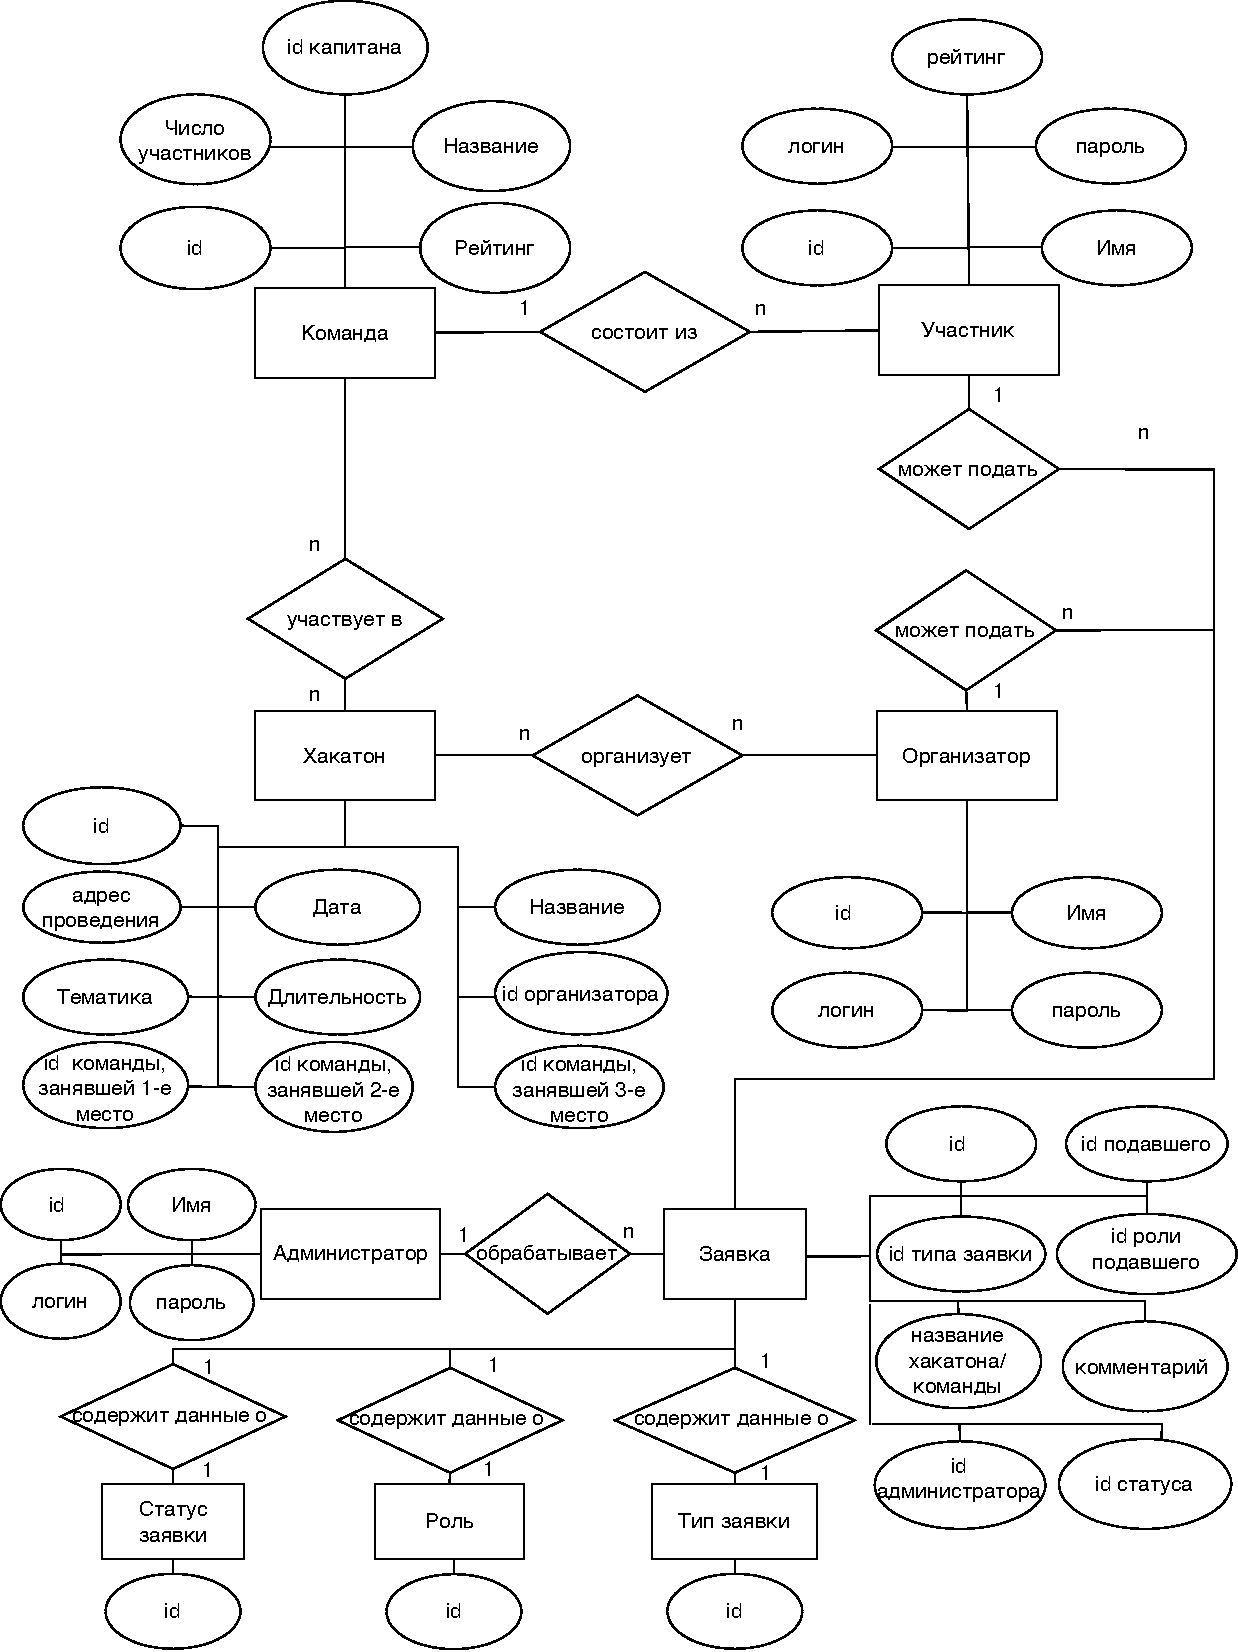
\includegraphics[page=1,scale=0.8]{assets/ER-Chen.drawio.pdf}
	\end{center}
	\caption{ER-диаграмма сущностей предметной области}
	\label{er-diagram}
\end{figure}

\section{Функционал приложения}

Приложение должно поддерживать следующий функционал:
\begin{itemize}
	\item авторизация пользователей;
	\item создание новых заявок и изменение информации об уже существующих;
	\item создание организаторами хакатонов;
	\item создание участниками команд и добавление в неё других участников;
	\item просмотр пользователями списков команд и событий.
\end{itemize}

% \section{Пользователи системы}

Для работы с системой обязательным этапом является прохождение авторизации. Пользователь может работать в системе под одной из следующих ролей:
\begin{enumerate}
	\item Участник -- пользователь, обладающий возможностями просмотра информации о событиях и командах, а также подачи заявок на создание команды или участие в команде.
	\item Капитан команды -- пользователь, обладающий возможностями добавления и удаления участников из команды и подачи заявки на участие команды в хакатоне.
	\item Организатор -- пользователь, обладающий возможностью создания хакатонов, приема заявок на участие команд в созданном им хакатоне, а также присвоения призовых мест командам.
        \item Администратор -- пользователь обладающий возможностью создавать и удалять заявки, удалять события, участников, а также просматривать информацию о событиях, участниках и командах.
\end{enumerate}

На рисунках \ref{use-case-participant}-\ref{use-case-admin} представлена диаграмма использования приложения в соответствие с ролями пользователей.

\begin{figure}[H]
	\begin{center}
		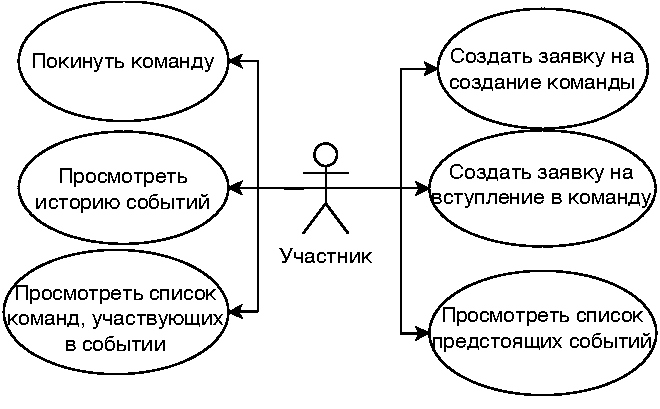
\includegraphics[page=1,scale=1]{assets/use-case-participant.drawio.pdf}
	\end{center}
	\caption{Use-case диаграмма участника}
	\label{use-case-participant}
\end{figure}

\begin{figure}[H]
	\begin{center}
		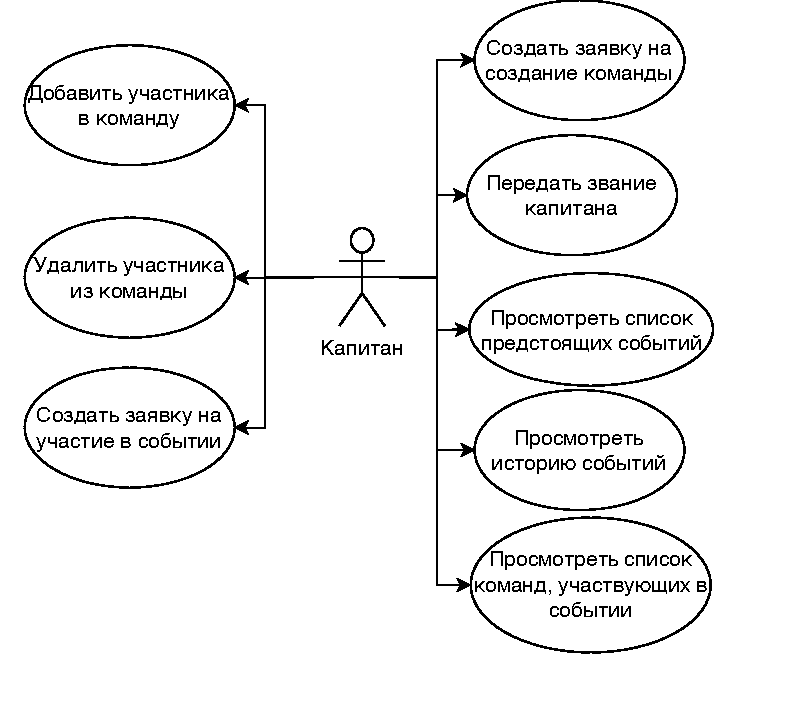
\includegraphics[page=1,scale=1]{assets/use-case-captain.drawio.pdf}
	\end{center}
	\caption{Use-case диаграмма капитана}
	\label{use-case}
\end{figure}

\begin{figure}[H]
	\begin{center}
		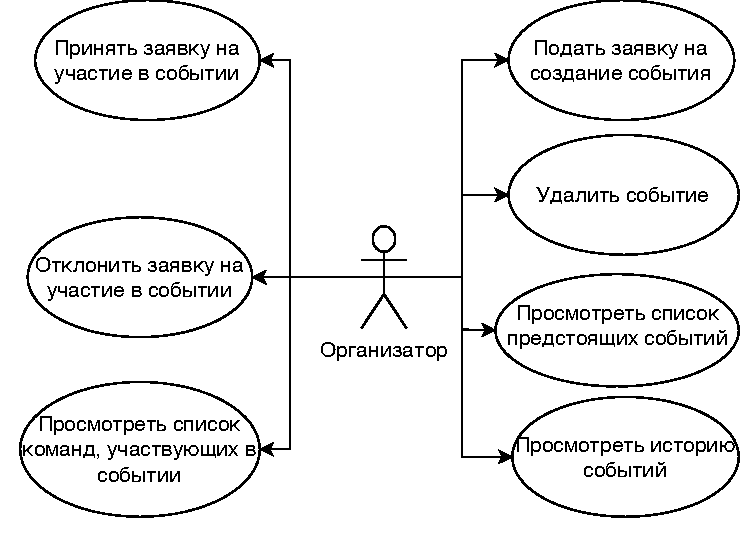
\includegraphics[page=1,scale=1]{assets/use-case-org.drawio.pdf}
	\end{center}
	\caption{Use-case диаграмма организатора}
	\label{use-case}
\end{figure}

\begin{figure}[H]
	\begin{center}
		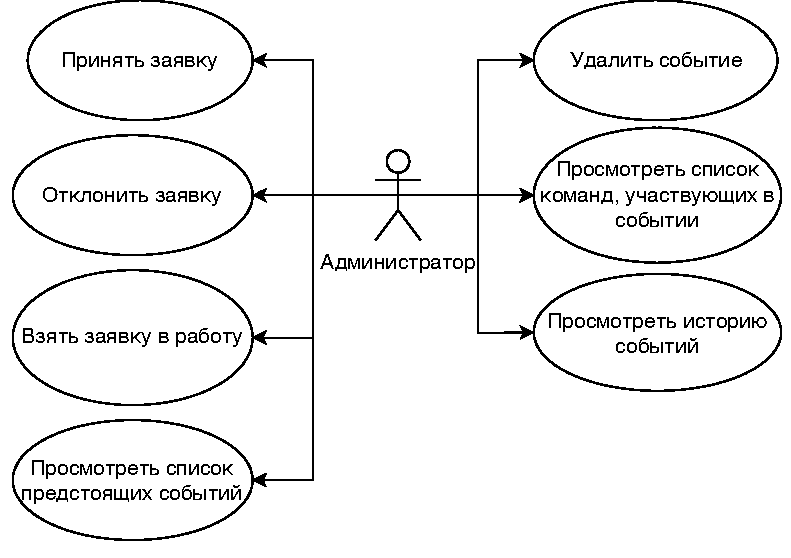
\includegraphics[page=1,scale=1]{assets/use-case-admin.drawio.pdf}
	\end{center}
	\caption{Use-case диаграмма администратора}
	\label{use-case-admin}
\end{figure}


\section{Анализ моделей баз данных}

\subsection{Иерархическая модель данных}

Иерархическая модель данных подразумевает что элементы, организованные в структуры, объединены иерархической или древовидной связью. В таком представлении родительский элемент может иметь несколько дочерних, а дочерний -- только один родительский.

Каждая вершина дерева соответствует типу сущности ПО.  Конечные вершины, то есть вершины, из которых не выходит ни одной дуги, называются листьями дерева. Каждая некорневая вершина связана с родительской вершиной иерархическим групповым отношением. Тип сущности характеризуется произвольным количеством атрибутов, связанных с ней отношением 1:1. Атрибуты, связанные с сущностью отношением 1:n, образуют отдельную сущность (сегмент) и переносятся на следующий уровень иерархии. Реализация связей типа n:m не поддерживается.

Существенным недостатком такой модели является то, что каждая сущность может относится только к одному родительскому сегменту. Таким образом при необходимости множественного отношения происходит дублирование данных, что может привести к нарушению логической целостности БД\thinspace\cite{db}.

\subsection{Сетевая модель данных}

Сетевая модель базы данных подразумевает, что у родительского элемента может быть несколько потомков, а у дочернего элемента -- несколько предков. Структура такой модели представлена в виде графа, причем каждая вершина графа хранит экземпляры сущностей (записи одного типа) и сведения о групповых отношениях с сущностями других типов. Каждая запись может хранить произвольное количество значений атрибутов (элементов данных и агрегатов), характеризующих экземпляр сущности. Для каждого типа записи выделяется первичный ключ – атрибут, значение которого позволяет однозначно идентифицировать запись среди экземпляров записей данного типа.

Связи между записями выполняются в виде указателей, т.е. каждая запись хранит ссылку на другую однотипную запись (или признак конца списка) и ссылки на списки подчинённых записей, связанных с ней групповыми отношениями. Таким образом, в каждой вершине записи хранятся в виде связного списка.

В этой модели связь 1:n между сущностями реализуется с помощью групповых отношений, а связи 1:n между атрибутами сущности -- в рамках записи. Для реализации связей типа n:m вводится вспомогательный тип записи и две связи 1:n. 

Физическая независимость не обеспечивается в сетевой модели данных, потому что наборы организованы с помощью физических ссылок. Помимо этого данная модель не обеспечивает независимость данных от программ. Эти недостатки помешали обрести ей широкое распространение из-за сложного проектирования и поддержки \cite{db}.

\subsection{Реляционная модель данных}

Реляционная модель данных является самой распространенной в использовании. В отличие от вышеописанных, в данной модели не существует физических отношений между сущностями. Хранение информации осуществляется в виде таблиц (отношений), состоящих из рядов и столбцов. Отношение имеет имя, которое отличает его от имён всех других отношений. Атрибутам реляционного отношения назначаются имена, уникальные в рамках отношения. Обращение к отношению происходит по его имени, а к атрибуту – по именам отношения и атрибута.

В реляционных моделях данных нет необходимости просматривать все указатели, что облегчает выполнение запросов на выборку информации по сравнению с сетевыми и иерархическими моделями. Это означает, что порядок записей не является важным, также как и порядок столбцов.

Каждая запись идентифицируется уникальной комбинацией атрибутов -- первичным ключом. Для связи между отношениями используется внешний ключ -- копия первичного или уникального ключа атрибута сторонней сущности. Таким образом можно реализовывать связь 1:n. Для обеспечения связи n:m вводится дополнительная сущность, атрибутами которой являются внешние ключи соответствующих сущностей.

Обработка данных осуществляется с помощью декларативного языка запросов SQL \cite{sql}. 

\subsection{Многомерная модель} Многомерная модель представляет данные как многомерные массивы (гиперкубы), использование которых позволяет получать различные срезы при аналитической обработке данных. Осями многомерной системы координат служат основные атрибуты анализируемого бизнес-процесса. На пересечениях осей измерений находятся данные, количественно характеризующие процесс, — меры \cite{postrel}.

\subsection{Объектно-ориентированная модель} Данная модель представляет из себя структуру, которую графически можно изобразить в виде дерева, узлами которого являются объекты. Базовыми понятиями являются: объекты, классы, методы, наследование, полиморфизм, инкапсуляция.

Спецификой объектно-ориентированной модели является то, что она поддерживает множественные группы, называемые ассоциированными множественными полями, а совокупность объединенных множественных полей называется ассоциацией. В объектно-ориентированной модели не накладываются требования на длину и количество полей в записях, что делает структуру таблиц более наглядной.
Таким образом, основным достоинством данной модели является возможность представления совокупности связанных реляционных таблиц в виде одной объектно-ориентированной таблицы. А недостатком является сложность обеспечения целостности и непротиворечивости данных, хранимых в ней \cite{postrel}. 

\section{Выбор модели базы данных}

В данном проекте будет использоваться реляционная модель данных, потому что в рамках проекта она обладает следующими преимуществами:
 
\begin{itemize}
	\item изложение информации осуществляется с помощью простых и понятных форм (таблиц);
	\item позволяет работать со структурированными данными, структура которых не подвергается частым изменениям;
	\item имеет возможность произвольного доступа к записям сущностей;
	\item исключает дублирование, реализуя связь между отношениями посредством внешнего ключа.
\end{itemize}

\section{Вывод из раздела}

В данном разделе был проведён анализ предметной области, построена её модель в виде ER-диаграммы, выделены ролевые модели системы, конкретизированы хранимые данные и их связь между собой, построены соответствующие диаграммы. Также был проведен анализ существующих на рынке решений, который позволил понять, какие особенности стоит добавить в разрабатываемый проект. Был осуществлен выбор модели базы данных.